

\section{Method}\label{sec:algorithm} 
Utilizing RGBD monocular streams captured by a Kinect camera, DynTCG seamlessly integrates recent advancements in differentiable rasterization with tracking flow and deformable fields\cite{yang2023deformable3dgs}. This innovative blend not only enhances the optimization process but also significantly improves the rendering quality. Moreover, our approach demonstrates remarkable performance in terms of storage efficiency. A visual summary of our methodology can be found in Fig.~\ref{fig:fig_2_overview}.

Our approach begins with the creation of an initial point cloud via depth back-projection, followed by the initialization of Gaussians. Concurrently, we project these Gaussians onto pixels and establish the warped relationship between Gaussian point clouds across frames using a pixel tracking method between consecutive frames. This results in the creation of warped Gaussians, which serve as a prior for the deformable network. The deformable network utilizes these warped Gaussians and time as inputs to estimate the changes in position and rotation of the Gaussians, thereby training temporal Gaussians. Furthermore, we introduce a novel compression scheme. This scheme significantly reduces storage needs, enabling the immersive viewing of high-fidelity human performances with a storage requirement of less than 2 MB per frame.

\subsection{Flow tracking}
Inspired by Instant-NVR~\cite{jiang2023instantnvr}, we aim to enhance the training speed and rendering effectiveness of the deform field by introducing a geometric constraint as a robust prior. While the ed node employed in Instant-NVR represents a powerful geometric prior, its integration into the Gaussian code proves to be challenging. Drawing further inspiration from the approach in dynamic nerf~\cite{gao2021dynamic}, which utilizes optical flow to provide prior information, we integrate optical flow into the Gaussian training pipeline. This involves calculating the $\delta x$ and $\delta y$ from optical flow derived from the 2D image, along with $\delta z$ information from the depth image. Through projection and back-projection calculations, we obtain a prior for the deform net.
\begin{figure}[t] 
	\begin{center} 
		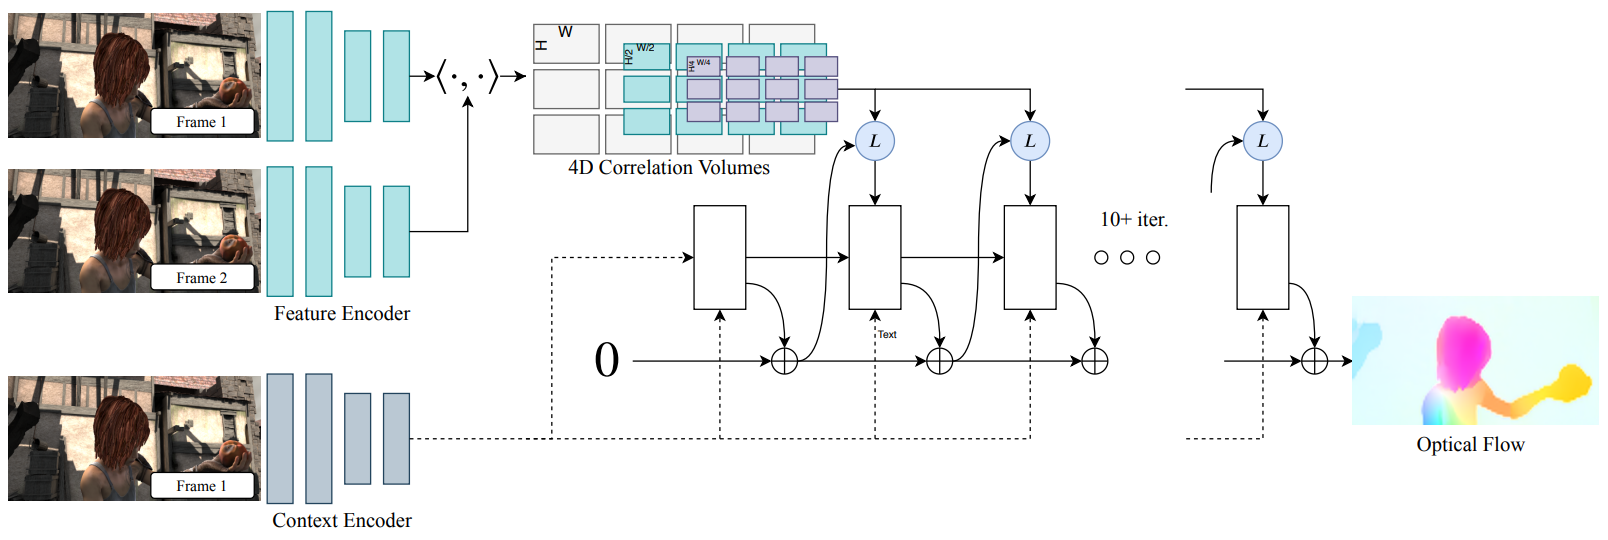
\includegraphics[width=\linewidth]{sec/fig/RAFT.png} 
	\end{center} 
    \vspace{-20pt}
    \caption{\noindent{\bf Pipeline of RAFT}: containing Feature Extractor \& Context Extractor, Visual Similarity Calculator and Updater}
    \label{fig:hello}
\end{figure}
We employ RAFT~\cite{10.1007/978-3-030-58536-5_24} as our method for optical flow tracking. RAFT comprises a Feature Extractor, Context Extractor, Visual Similarity Calculator, and Updater to optimize the flow tracking process. The pipeline of RAFT is shown in Fig.~\ref{fig:hello}.
\\
\textbf{Feature Extractor \& Context Extractor } extract features from two images, followed by the extraction of semantic information from one of the images.
\\
\textbf{Visual Similarity Calculator }constructs a 4D correlation volume by calculating the dot product between feature vectors.
\\
\textbf{Updater }updates and refines flow tracking by iteratively searching the correlation volume based on current optical flow estimates.

\begin{figure}[b]
	\centering
	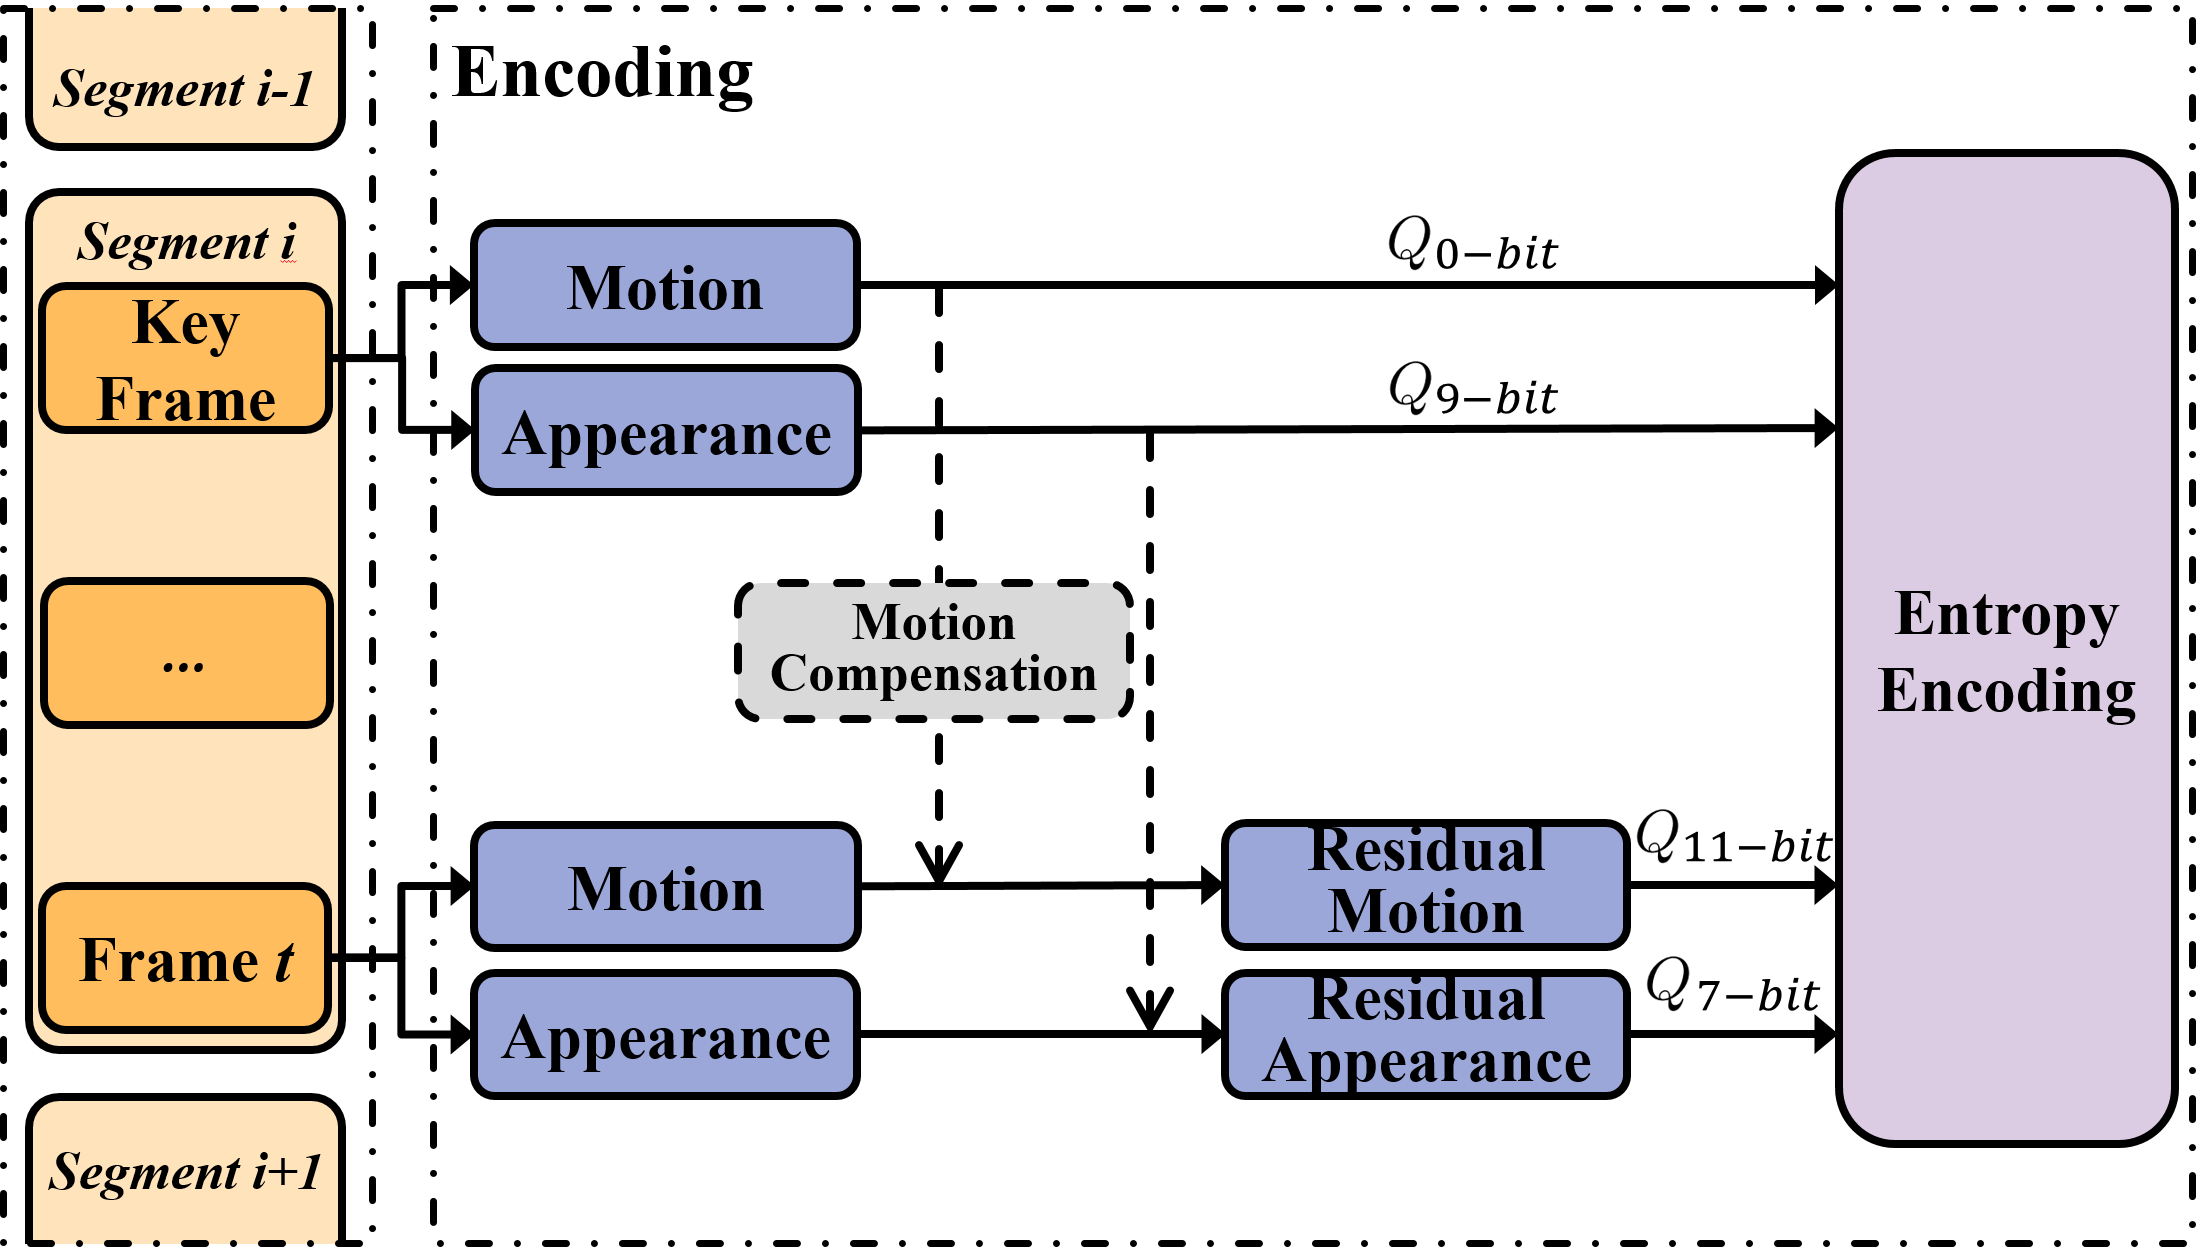
\includegraphics[width=\linewidth]{sec/fig/encoding.png}
	\vspace{-20pt}
	\caption{Illustration of residual encoding strategy for DynTCG.}
	\label{fig:encoding}
\end{figure}
\subsection{Compact 4D Gaussians}
After Gaussian optimization, we dump the Gaussian splat points and the deformation network into separate frame Gaussian splat points. However, storage of 64-dimensional with a 3-order sh coefficient takes large disk storage, making it hard to store long dynamic sequences. To address this, we present a Residual Compression method as shown in Fig.~\ref{fig:encoding}, including residual computation, quantization, and RANS encoding. 

\noindent{\bf Residual Compression}
For dynamic sequences, adjacent frames share similar Gaussian point parameters in a set of frames. We split the whole sequence into several segments and the object's movement is relatively small, then we compute the residual data between each frame and the first frame, such that the residual data distribution range of data will be much smaller. Then we apply compression separately to motion and appearance. 

\noindent{\bf Quantization}
As for the residual data, we perform quantization separately to the delta position and delta appearance. As motion needs higher precision to maintain rendering quality, we adopt a lower quantization bit on the position attribute. We need to ensure the precision for the first frame, so we do not perform quantization to the first frame position and perform 9-bit quantization to appearance to ensure the base frame precision. For other frames in this segment, we adopt 11-bit quantization to delta position and 7-bit quantization to delta appearance. 

\noindent{\bf RANS Encoding}
After quantization of the float number to an integer number, we perform RANS encoding to compress the data. This entropy encoding system encodes each attribute by calculating the numerical distribution frequency and finally encodes the attribute to an integer stream. 
By using our residual encoding method, we could compress the Gaussian point cloud efficiently by 20 times on the storage, which addresses long dynamic sequences on low disk storage and fast data transport. 

\section{Implementation Details}\label{sec:detail} 

Firstly, for data obtained from HyperNeRF\cite{park2021hypernerf} and DynamicNeRF\cite{gao2021dynamic} datasets, we leverage the state-of-the-art single-image depth estimation\cite{Ranftl2022} to estimate the input depth. Our approach to the deformable field is inspired by the work of Ziyi Yang\cite{yang2023deformable3dgs} and is based on a broad framework of 3D Gaussians\cite{kerbl3Dgaussians}.

Regarding the training process, we conducted a total of 40,000 iterations. In the initial 3,000 iterations, we solely trained the 3D Gaussians to attain relatively stable positions and shapes. Following this phase, we commenced the joint training of both the 3D Gaussians and the deformation field. A single Adam optimizer\cite{kingma2017adam}, was utilized for optimization purposes.
During compression, we first quantize the appearance attributes, then fix these parameters and fine-tune motion $p$ and $q$ of 4D Gaussians over an additional 1000 iterations. Afterward, we quantize the motion. To mitigate the influence of quantization on the outcomes, We apply different precision levels for various attributes to balance storage and quality.

All the experiments were done on 4 Nvidia 2080Ti.


% We implement our framework using PyTorch [32] and modify the differentiable Gaussian rasterization by incorporating depth visualization. For training, we conducted training for a total of 40k iterations. During the initial 3k iterations, we solely trained the 3D Gaussians to attain relatively
% stable positions and shapes. Subsequently, we jointly train
% the 3D Gaussians and the deformation field. For optimization, a single Adam optimizer [17] is used but with a different learning rate for each component: the learning rate of
% 3D Gaussians is exactly the same as the official implementation, while the learning rate of the deformation network
% undergoes exponential decay, ranging from 8e-4 to 1.6e-6.
% Adam’s β value range is set to (0.9, 0.999). Experiments
% with synthetic datasets were all conducted against a black
% background and at a full resolution of 800x800. All the experiments were done on an NVIDIA RTX 3090.
